\section{Methodology}
\begin{frame}{Methodology}
    \framesubtitle{Overview}
    The proposed methodology is structured into two phases:
    \vspace*{0.3cm}
    \begin{itemize}
        \item \textbf{Phase I: Protocol and Architecture Design}\\
        Formal specification of a Taproot-based scheme for document batching and verification.
        \vspace*{0.2cm}
        \item \textbf{Phase II: Proof of Concept and Performance Estimations}\\
        Design of a Proof of Concept and analytical estimation of verification complexity and on-chain costs.
    \end{itemize}
\end{frame}



\begin{frame}{Methodology}
    \framesubtitle{Verification Goals}
    The proposed protocol supports three verification objectives:
    \vspace*{0.2cm}
    \begin{itemize}
        \item \textbf{Integrity}: The document content has not been altered.
        \item \textbf{Authenticity}: The document was issued by the claimed organization.
        \item \textbf{Revocation}: The document has not been revoked.
    \end{itemize}
    \vspace*{0.3cm}
    Verification is performed \textbf{off-chain} using a \textbf{validation proof} provided  together with the document.\\
    \vspace*{0.1cm}
    The protocol is structured into two stages: \textbf{issuance} and \textbf{verification}.
\end{frame}


\begin{frame}{Phase I}
\framesubtitle{Issuance}
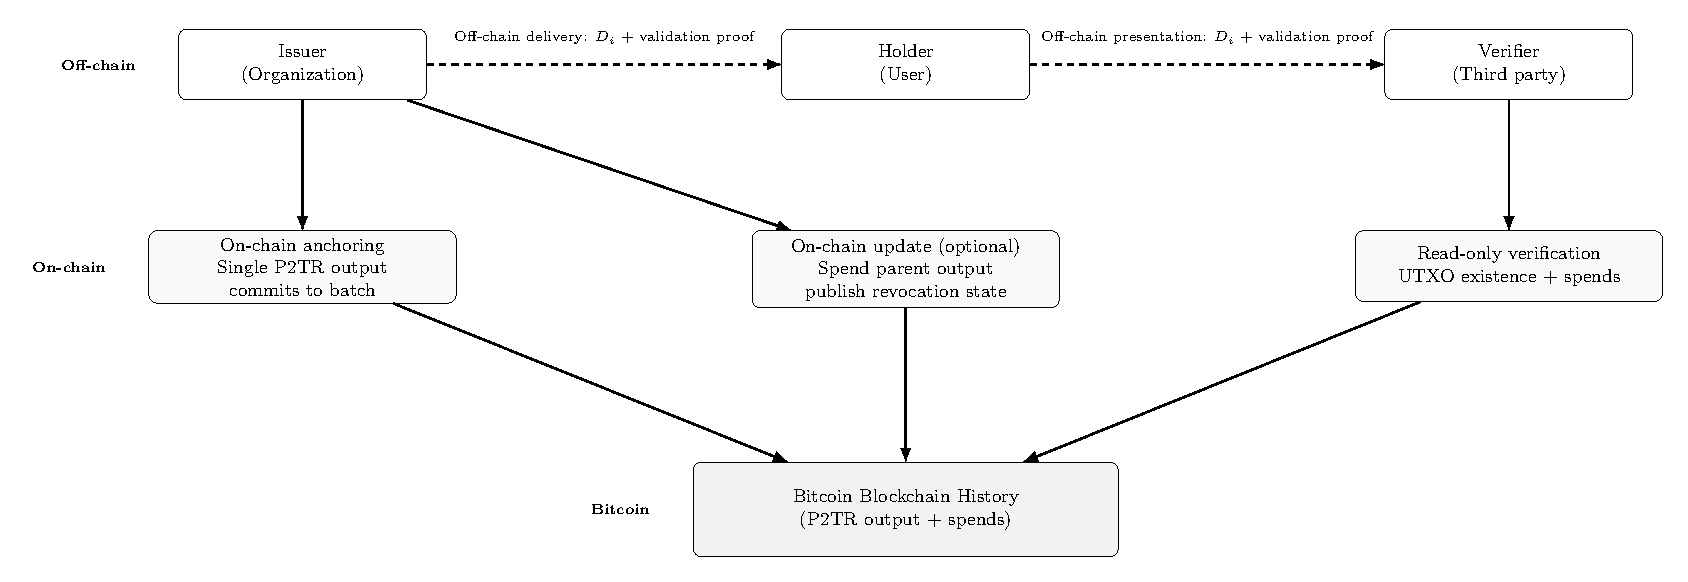
\includegraphics[width=1.\textwidth,height=0.6\textheight]{figures/figure1.pdf}
\end{frame}

\begin{frame}{Phase I}
    \framesubtitle{Privacy via MAST}
    \begin{block}{Privacy Preserved}
        Each script leaf contains the document hash and verification logic and is intentionally non-spendable.
        Other documents in the batch remain hidden.
    \end{block}   
    \vspace*{0.3cm}
    \centering
    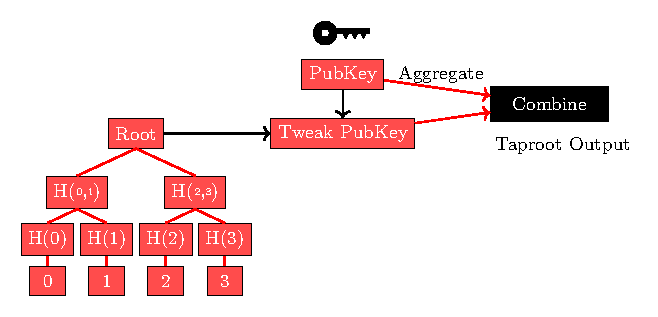
\includegraphics[width=0.7\textwidth]{figures/mast.pdf}

\end{frame}



\begin{frame}{Phase I}
\framesubtitle{Cryptographic Binding (Taproot)}

\textbf{Script leaf structure}
\[
\text{leaf}_i = \big( \; h_i \; \| \; \mathcal{L} \; \big),
\quad
h_i = \mathrm{SHA256}(D_i)
\]
where $h_i$ is the document hash and $\mathcal{L}$ represents non-spendable verification logic.

\vspace*{0.1cm}

\textbf{Merkle commitment}
\[
m = \mathrm{MerkleRoot}(\{\text{leaf}_1,\dots,\text{leaf}_N\})
\]


\end{frame}

\begin{frame}{Cryptographic Binding (Taproot)}


\textbf{Taproot key derivation}
\[
Q = P_{\text{btc}} + \mathrm{H}_{\text{TapTweak}}(P_{\text{btc}} \| m)\,G
\]
where $P_{\text{btc}}$ is the issuer’s Bitcoin public key used for Taproot output creation.\\
\vspace*{0.1cm}
\textbf{Document authenticity}
\[
\sigma_i = \mathrm{Sign}(sk_{\text{doc}},\, h_i),
\quad
\mathrm{Verify}(pk_{\text{doc}},\, h_i,\, \sigma_i)
\]
where $(pk_{\text{doc}}, sk_{\text{doc}})$ is the key pair used exclusively for document signing.
\end{frame}

\begin{frame}{Phase I}
\framesubtitle{Verification (Off-chain)}
\centering
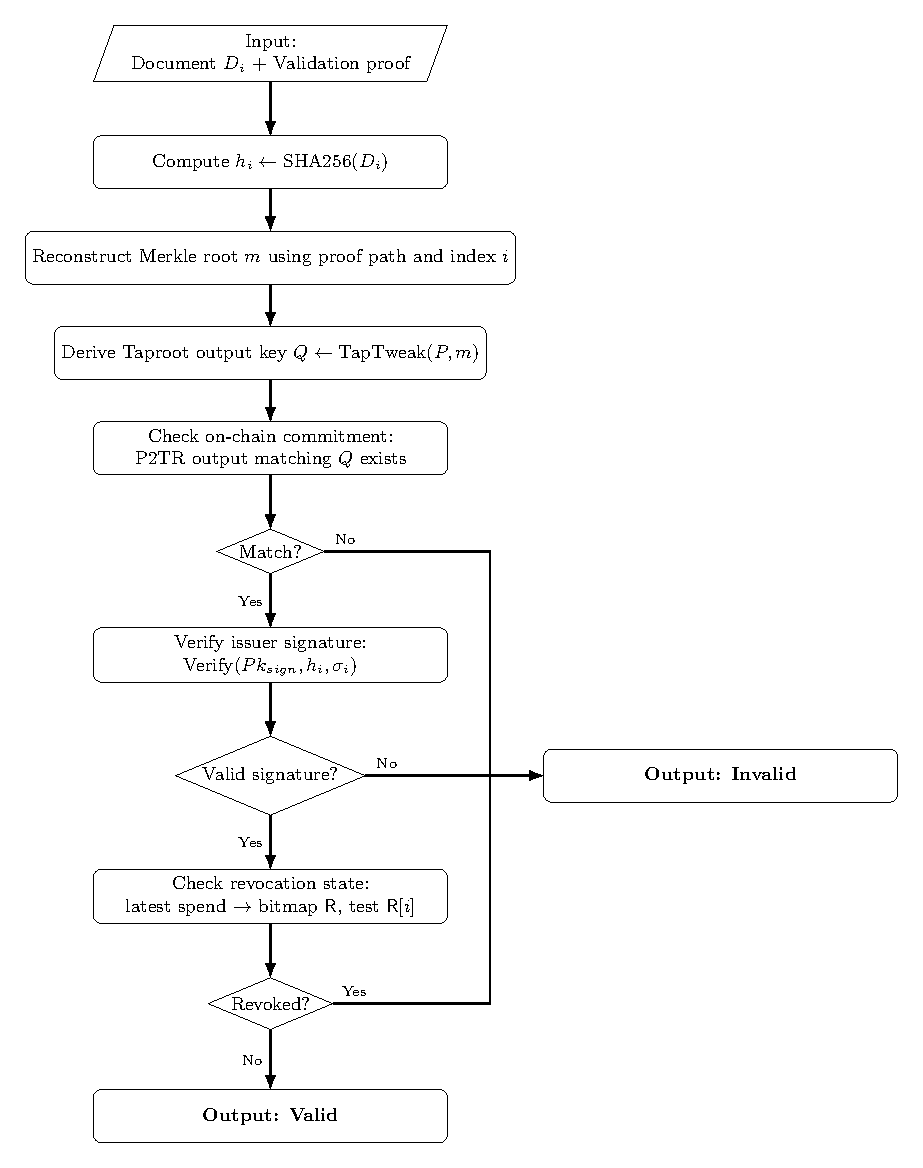
\includegraphics[width=1.5\textwidth,height=0.8\textheight,keepaspectratio]{figures/figure2.pdf}
\end{frame}


\begin{frame}{Phase I}
\framesubtitle{Revocation (On-chain State Update)}
Revocation is modeled as an \textbf{on-chain state update} rather than a modification of past data.\\
\vspace*{0.2cm}
\begin{itemize}
    \item The batch commitment is anchored in a P2TR output and cannot be edited after publication.
    \item To revoke, the issuer \textbf{spends} the current P2TR output and creates a new child output that commits to:
    \begin{itemize}
        \item the same batch structure, and
        \item a revocation state (e.g., a bitmap indexed by document position).
    \end{itemize}
    \item Verifiers follow the spending chain to the \textbf{latest} output and read the revocation state to decide validity.
    \item Details on indexing and state encoding are \textbf{to be analyzed}.
\end{itemize}
\end{frame}
\begin{frame}{Phase II}
\framesubtitle{Proof of Concept and Evaluation Scope}
This phase addresses objectives (d) and (e) through a controlled and analytical approach.
\vspace*{0.2cm}
\begin{itemize}
    \item \textbf{Proof of Concept (PoC) Design}:\\
    Specification of a reference workflow demonstrating issuance, verification, and revocation using the proposed protocol.
    \vspace*{0.2cm}
    \item \textbf{Experimental Context}:\\
    The PoC is designed for execution on Bitcoin \textbf{Signet/Testnet} environments to avoid real network costs.
\end{itemize}
\end{frame}

\begin{frame}{Phase II}
\framesubtitle{Metrics and Cost Analysis}
The protocol is evaluated through analytical metrics focusing on scalability and on-chain cost.
\vspace*{0.3cm}
\begin{columns}[T]
\column{0.5\textwidth}
\textbf{Scalability}
\begin{itemize}
    \item Evaluated as a function of the batch size $N$.
    \item Verification complexity is bounded by $\mathcal{O}(\log N)$ due to Merkle tree inclusion proofs.
\end{itemize}

\column{0.5\textwidth}
\textbf{On-chain Cost}
\begin{itemize}
    \item Estimated in \textbf{vBytes}.
    \item Includes anchoring and revocation transactions.
\end{itemize}
\end{columns}

\vspace*{0.4cm}
The analysis highlights trade-offs between privacy, scalability, and network cost.
\end{frame}
